\documentclass[lang=cn,11pt,a4paper,cite=authornum]{paper}

\title{大数据技术基础 实验一 \\ 实验报告}
\author{毛子恒 \\ 2019211397}
\institute{北京邮电大学\ 计算机学院}

\date{\zhtoday}

% 本文档命令
\nocite{*}

\begin{document}

\maketitle

\part{实验一(一)}

\section{概述}

\subsection{实验目的}

\begin{enumerate}
    \item 了解华为云基础操作;
    \item 购买华为云ECS;
    \item 掌握华为云服务器操作。
\end{enumerate}

\subsection{实验步骤}

\begin{enumerate}
    \item 购买4个ECS实例;
    \item 创建OBS桶,获取访问密钥和endpoint。
\end{enumerate}

\section{实验结果及分析}

\paragraph{购买ECS}

登录华为云控制台,依照实验指导书的步骤购买ECS,购买结果如\figref{fig:ECS}。

\begin{figure}[!htb]
    \centering
    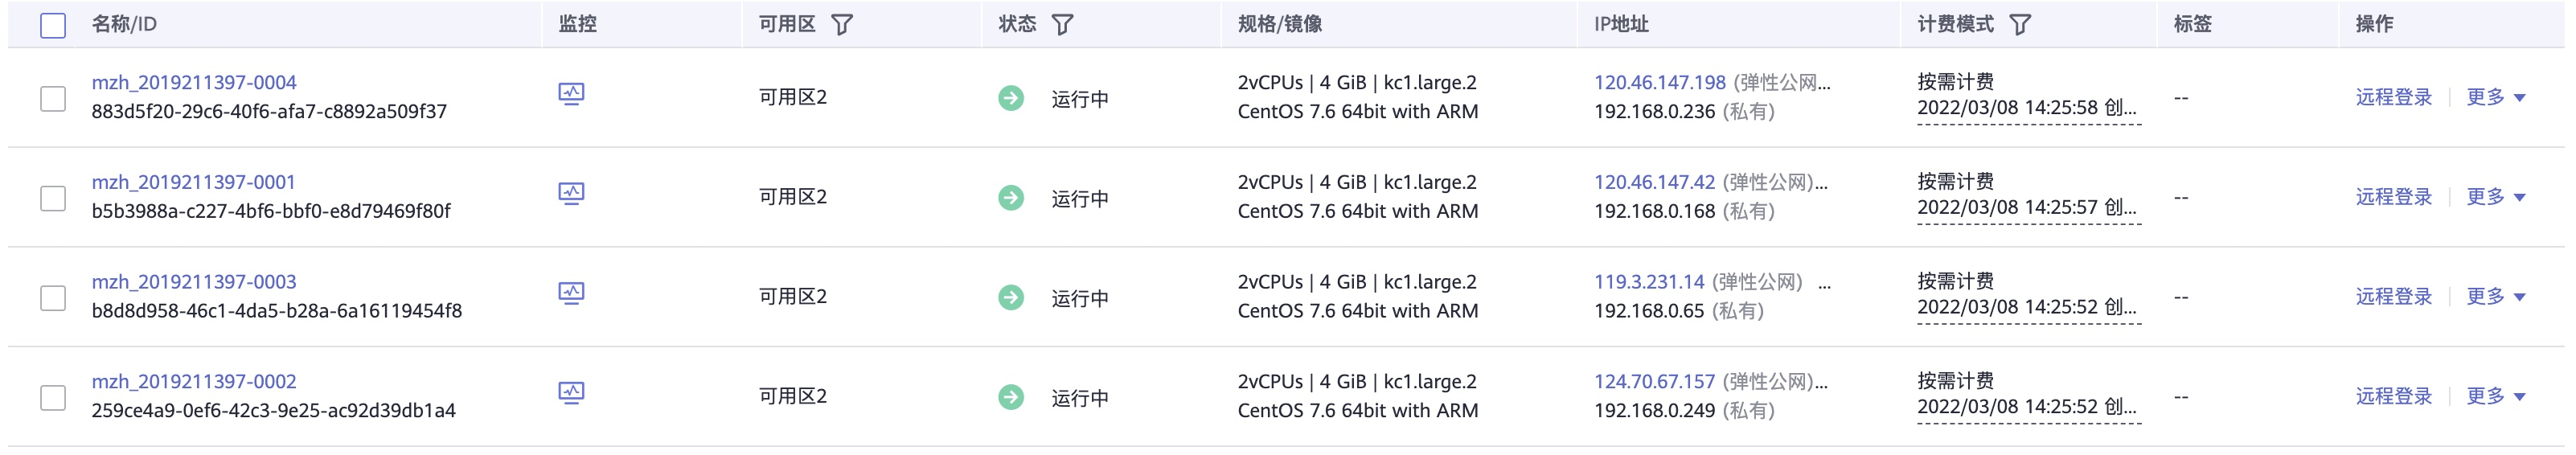
\includegraphics[width=\textwidth]{./images/ECS.jpg}
    \caption{购买ECS\label{fig:ECS}}
\end{figure}

\paragraph{创建OBS桶}

依照实验指导书的步骤创建OBS桶,结果如\figref{fig:OBS}。

\begin{figure}[!htb]
    \centering
    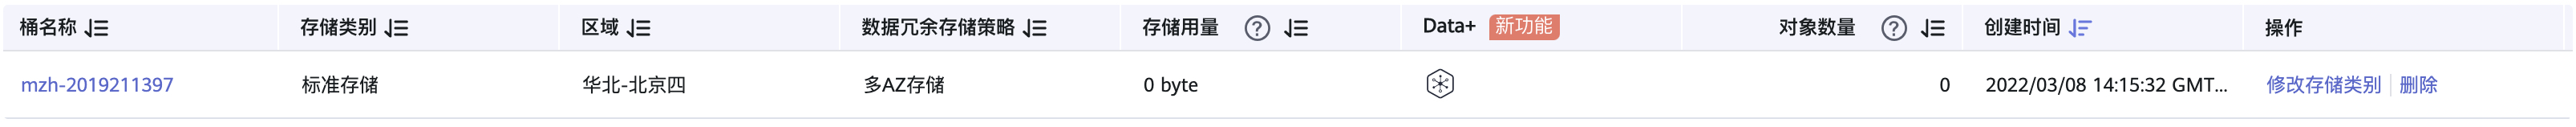
\includegraphics[width=\textwidth]{./images/OBS.jpg}
    \caption{创建OBS桶\label{fig:OBS}}
\end{figure}

\paragraph{获取访问密钥和endpoint}

依照实验指导书的步骤获取访问密钥和endpoint,结果如\figref{fig:key}和\figref{fig:endpoint}。

\begin{figure}[!htb]
    \centering
    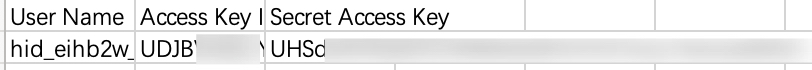
\includegraphics[width=0.7\textwidth]{./images/key.jpg}
    \caption{访问密钥\label{fig:key}}
\end{figure}

\begin{figure}[!htb]
    \centering
    
\includegraphics[width=0.4\textwidth]{./images/endpoint.jpg}
    \caption{endpoint\label{fig:endpoint}}
\end{figure}

\section{实验总结}

本次实验中我基本熟悉了华为云ECS的基本操作,创建了ECS和OBS实例,为之后的实验做了准备工作。

\part{实验一(二)}

\section{概述}

\subsection{实验目的}

\begin{enumerate}
    \item 学习搭建Hadoop集群;
    \item 学习创建Maven工程;
    \item 掌握HDFS文件读写操作。
\end{enumerate}

\subsection{实验步骤}

\begin{enumerate}
    \item Hadoop集群搭建;
    \item 创建Maven工程;
    \item Java实现HDFS文件读写。
\end{enumerate}

\section{实验结果及分析}

\paragraph{Hadoop集群搭建}

依照实验指导书的步骤搭建Hadoop集群,有以下几点需要注意:

\begin{enumerate}
    \item 将主机名和IP替换成自己的主机名和IP;
    \item 执行命令或者配置环境变量时,注意删去多余的空格,比如实验指导书中,设置
    \mintinline{text}{hadoop-env.sh}的环境变量时,\mintinline{text}{JAVA_HOME}的路径中有空格,需要删除。
    \item 部分图片与文字描述不符,以文字为准;
    \item 设置\mintinline{text}{core-site.xml}时,\mintinline{text}{hadoop.tmp.dir}属性的值应该为\mintinline{text}{/home/modules/hadoop-2.7.7/tmp}。
    \item \mintinline{text}{scp}命令的前一个参数为\mintinline{text}{/home/modules/hadoop-2.7.7},注意不要多一个\mintinline{text}{/},否则会将子文件夹拷贝过去。
    \item 配置出错和关闭服务器之前执行\mintinline{text}{stop-all.sh}。
    \item 如果node1中也有DataNode,首先检查\mintinline{text}{slaves}文件里应该没有node1,并且执行\mintinline{text}{hdfs namenode -format}且重启。
\end{enumerate}

成功搭建并启动Hadoop集群的结果如\figref{fig:jps},主机有四个进程,分别是主次NameNode、资源管理和Jps,从机有三个进程,分别是节点管理、Jps和DataNode。

\begin{figure}[htbp]
    \centering
    \subfigure[node1]{
        \begin{minipage}[t]{0.45\linewidth}
            \centering
            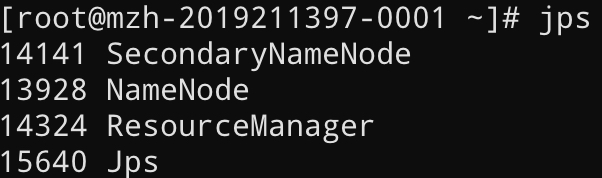
\includegraphics[width=\linewidth]{./images/node1.jpg}
        \end{minipage}
    }
    \subfigure[node2]{
        \begin{minipage}[t]{0.45\linewidth}
            \centering
            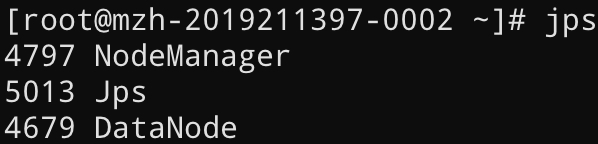
\includegraphics[width=\linewidth]{./images/node2.jpg}
        \end{minipage}
    }
    \caption{在node1和node2中执行jps命令的结果\label{fig:jps}}
\end{figure}

\paragraph{创建Maven工程}

依照实验指导书的步骤创建Maven工程,注意如果是全新的环境,在创建项目时需要自行下载一个1.8版本的SDK。

\paragraph{Java实现HDFS文件读写}

依照实验指导书的步骤编写Java代码,有以下几点需要注意:

\begin{enumerate}
    \item 使用IDEA自动添加import时,可能会导入Java自定义的虚类,需要改成Hadoop实现的子类,如\figref{fig:import}。
    \item 所有方法改为静态方法。
    \item 对于\mintinline{text}{log4j: WARN No appenders could be found for logger}的报错,需要增加一个log4j的配置文件,参考\href{https://www.jianshu.com/p/ea2de77eb9d4}{这里}。
    \item 服务器需要设置安全组,开放8020端口进行NameNode的RPC调用,50010端口用于DataNode的数据传输,还有一些其他的Web端口用于查看状态,具体如\figref{fig:safegroup}。
\end{enumerate}

\begin{figure}[!htb]
    \centering
    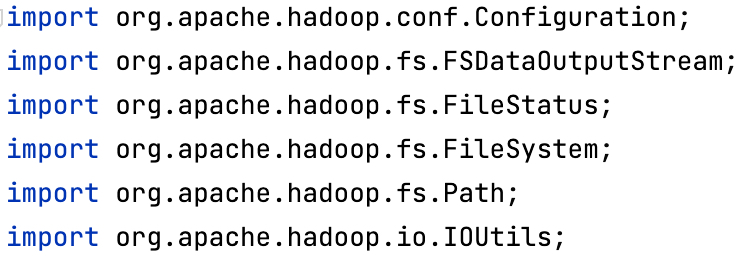
\includegraphics[width=0.6\textwidth]{./images/import.jpg}
    \caption{import\label{fig:import}}
\end{figure}

\begin{figure}[!htb]
    \centering
    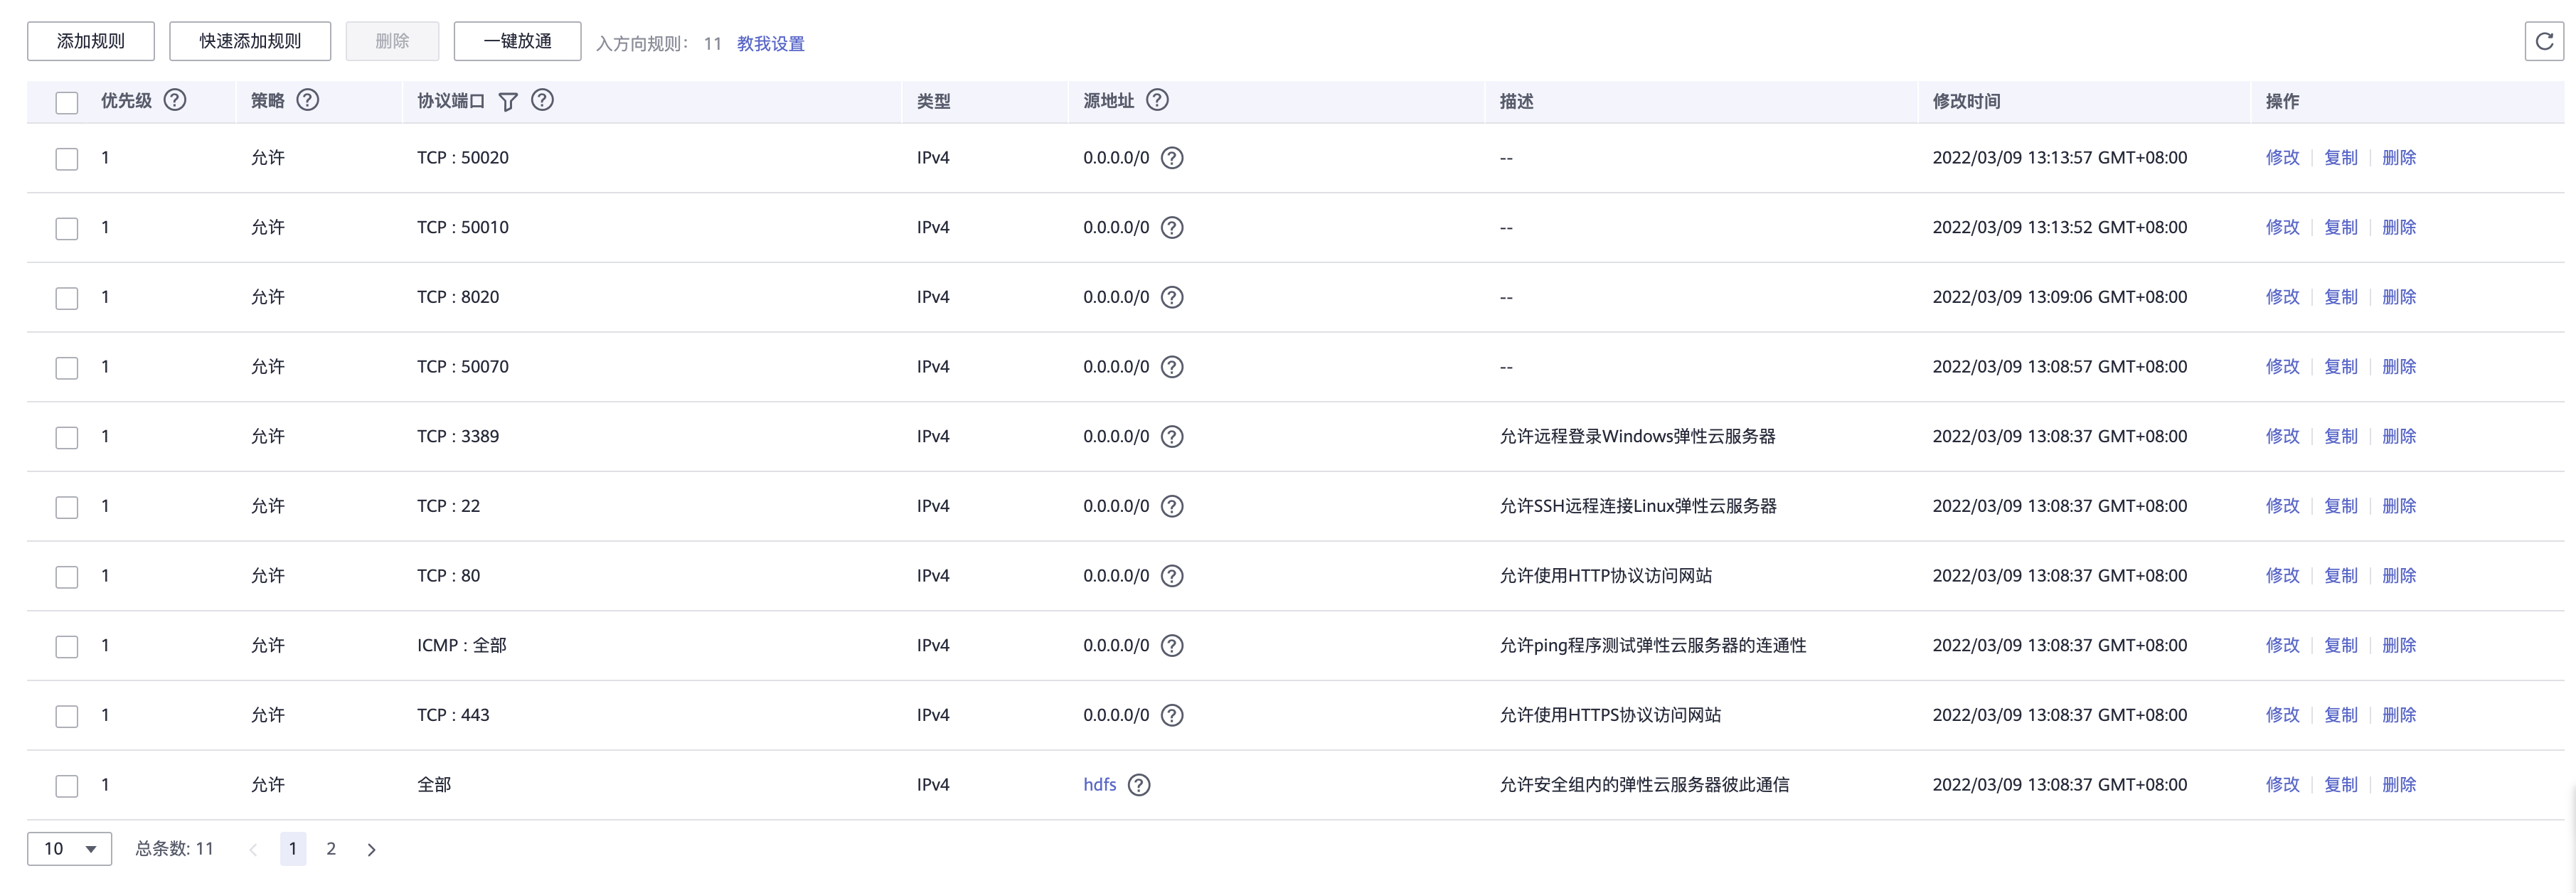
\includegraphics[width=\textwidth]{./images/safegroup.jpg}
    \caption{安全组\label{fig:safegroup}}
\end{figure}

代码运行结果如\figref{fig:result1},首先查看HDFS目录为空,之后上传了一个文件,又写入了一个文件\mintinline{text}{mzh_2019211397.txt},将刚才写入的文件下载下来,再查看HDFS的根目录,现在有两个文件。

\begin{figure}[!htb]
    \centering
    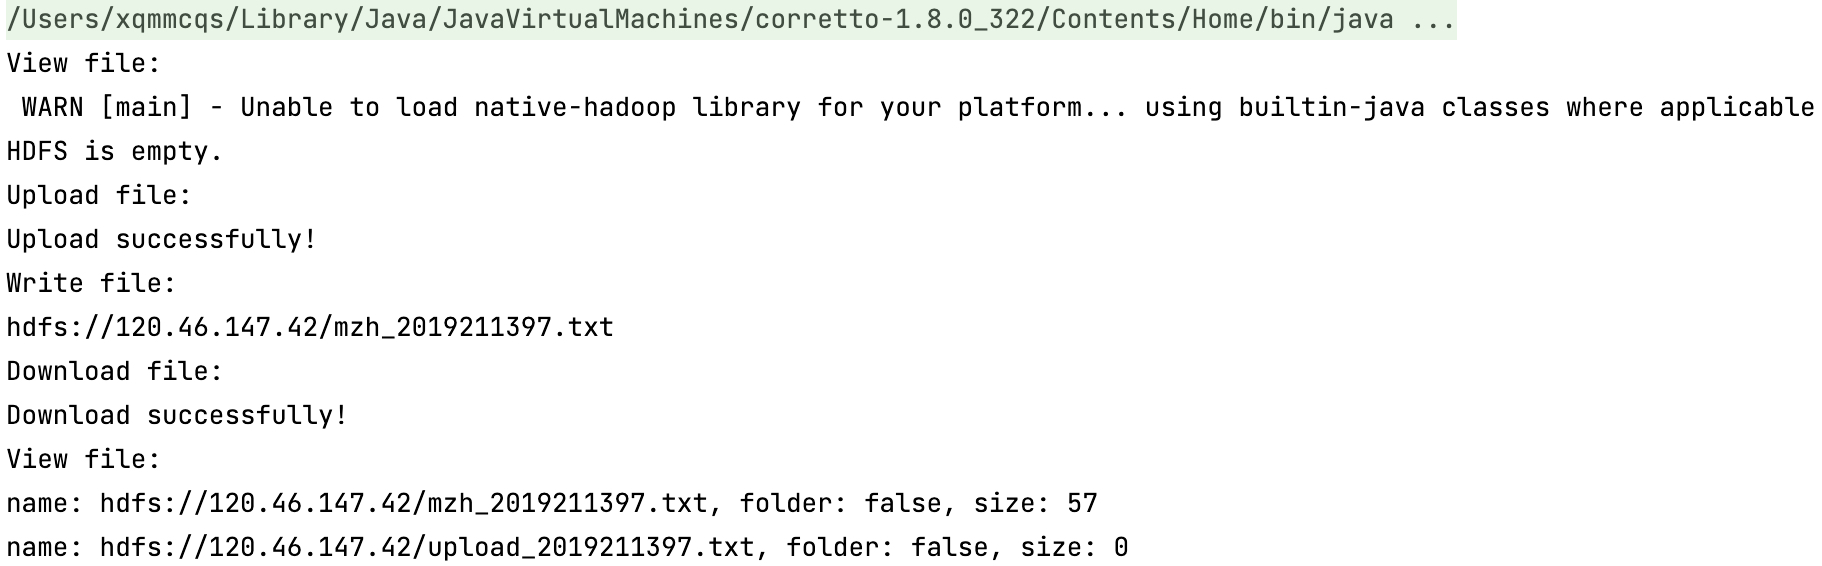
\includegraphics[width=\textwidth]{./images/result1.jpg}
    \caption{运行结果\label{fig:result1}}
\end{figure}

下载完成的文件如\figref{fig:result2},内容为我们代码中刚刚写入的。

\begin{figure}[!htb]
    \centering
    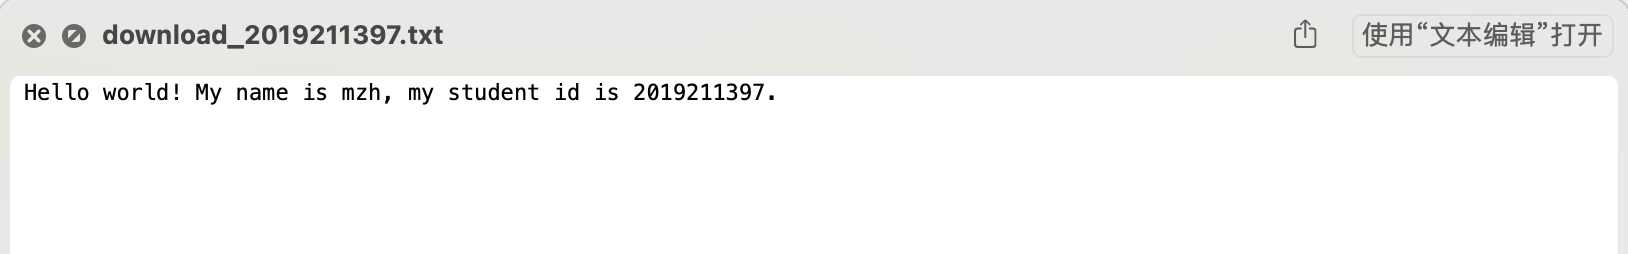
\includegraphics[width=\textwidth]{./images/result2.jpg}
    \caption{下载的文件\label{fig:result2}}
\end{figure}

\section{实验总结}

本次实验中我搭建了Hadoop集群,并且编写Java代码访问HDFS,进行了基本的文件操作。经过这次实验,我对Hadoop基本概念和特性有了更深的体会,同时增强了信息获取能力和Java代码能力。

\end{document}
